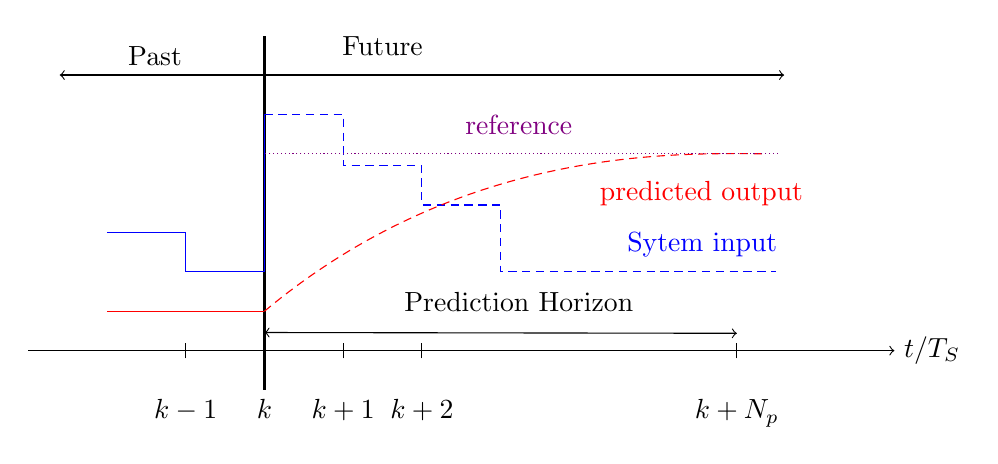
\begin{tikzpicture}
	% Timeline
	\draw[->] (-3, 0) -- (8, 0) node[right] {$t/T_S$};
	
	% Past/Future divider
	\draw[thick] (0, -0.5) -- (0, 4);
	\node[above] at (-1.39, 3.5) {Past};
	\node[above] at (1.5, 3.62) {Future};
	
	% Time axis labels
	\foreach \x/\label in {-1/k-1, 0/k, 1/k+1, 2/k+2, 6/k+N_p} {
		\draw (\x, -0.1) -- (\x, 0.1);
		\node[below] at (\x, -0.5) {$\label$};
	}

	% Arrows from past/future
	\draw[<-] (-2.6, 3.5) -- (0, 3.5);
	\draw[->] (0, 3.5) -- (6.6, 3.5);

  \draw[blue] (-2,1.5) -- (-1,1.5) -- (-1,1) -- (0,1) -- (0,3);

  \draw[densely dashed, blue] (0,3) -- (1,3) -- (1,2.35) -- (2,2.35) -- (2,1.85) -- (3,1.85) -- (3,1) -- (6.5,1);
  \draw[red] (0,0.5) -- (-2,0.5);
  \draw[densely dashed, red] (0,0.5) .. controls (2.56,2.64) and (5.34,2.5) .. (6.37,2.5);
  \draw[violet, densely dotted] (6.52,2.5) -- (0,2.5);
  \node[text=blue] at (5.56,1.34) {Sytem input};

  \node[text=red] at (5.55,2) {predicted output};

  \node[text=violet] at (3.23,2.87) {reference};

  \node[above] at (3.23, 0.37) {Prediction Horizon};
  \draw[<->] (0, 0.23) -- (6, 0.22);
\end{tikzpicture}